\documentclass{article}

% NeurIPS 2026 style (official kit, user-provided). Workshop options available:
%   \usepackage[sglblindworkshop]{neurips_2026}  + \workshoptitle{...}
%   \usepackage[dblblindworkshop]{neurips_2026}  + \workshoptitle{...}
% TODO(user/submission): switch to the workshop option matching ATTRIB's review
% policy and add [final] for camera-ready. [preprint] until then.
\usepackage[preprint]{neurips_2026}
\workshoptitle{ATTRIB: Workshop on Attributing Model Behavior at Scale}

\usepackage[utf8]{inputenc}
\usepackage[T1]{fontenc}
\usepackage{hyperref}
\usepackage{url}
\usepackage{booktabs}
\usepackage{amsfonts}
\usepackage{amsmath}
\usepackage{nicefrac}
\usepackage{microtype}
\usepackage{graphicx}
\usepackage{xspace}

% Consistent terminology macros (Steinhardt: one term per concept, everywhere)
\newcommand{\afirst}{\textsc{A-first}\xspace}
\newcommand{\bfirst}{\textsc{B-first}\xspace}
\newcommand{\interleaved}{\textsc{Interleaved}\xspace}
\newcommand{\score}{$S$\xspace}

\title{Training History Shapes Value Generalization\\in Language Models}

% TODO(user): authorship + affiliation decision pending (PROJECT.md Step 6 / "your list" item 5).
\author{
    Author TBD \\
    Affiliation TBD \\
    \href{mailto:tbd@tbd.tbd}{tbd@tbd.tbd}
}

\begin{document}

\maketitle

\begin{abstract}
% Farquhar 5-sentence structure (ml-paper-writing skill). Calibrated to current
% evidence; TODO-MATRIX comments mark the two upgrade points for n=8 locked-battery
% numbers. No claim below exceeds committed results.
The causal effect of an alignment training example depends on \emph{when} in training
it is encountered: we show that language models fine-tuned on identical conflicting
alignment datasets generalize to opposing values depending only on presentation order.
Training-data attribution methods and alignment data curation typically treat training
sets as unordered collections --- an assumption that cannot be tested without a control
prior comparisons lack: verification that the competing signals are independently
capable of installing their values. In a controlled conflicting-value testbed with
matched, equipotence-verified demonstration pools, we intervene only on curriculum
order --- with every ordering ending in an identical value-neutral washout phase --- and
measure held-out conflict behavior under blinded labeling. Sequential training exhibits
total recency dominance: the operative value reverses completely (per-seed score
$+1.0\!\to\!-1.0$) within ${\sim}8$ optimizer steps of the conflicting phase beginning,
in both directions and on every seed tested,
% TODO-MATRIX: "on every seed tested" -> exact n=8 statement + sign-flip p-value
and the resulting difference persists through the shared final phase, while interleaved
exposure produces fragmented, seed-varying policies rather than an average.
% TODO-MATRIX: persistence sentence gets endpoint means + paired p at n=8
We further isolate a supervision-format confound with direct attribution consequences:
value content trained as plain next-token prose exerts \emph{no} behavioral leverage
against completion-supervised demonstrations --- which won 43 of 43 decisive held-out
outputs regardless of order --- so na\"ive specification-versus-demonstration
comparisons manufacture spurious order-invariance. Attribution that ignores training
order can misattribute which data made a model's values.
\end{abstract}

\section{Introduction}

Training-data attribution methods typically treat a model's training set as an
unordered collection: an example's causal contribution to the final model is assumed
independent of \emph{when} in training it was encountered. Recent attribution theory
drops this permutation-invariance assumption on formal grounds
\citep{wang2024temporal}; whether it fails \emph{behaviorally} --- whether the same
alignment data, reordered, produces a model with different values --- has not been
tested directly. We test it.

We construct a controlled testbed in which two alignment datasets conflict:
matched prompt-for-prompt, they differ only in which of two competing institutional
values each response enacts. After verifying that each dataset alone reliably installs
its value (a precondition prior work skips, and without which order comparisons are
uninterpretable), we fine-tune models on the \emph{identical combined data} under three
curricula --- \afirst, \bfirst, and \interleaved --- each ending in a shared,
value-neutral washout phase, and measure which value governs behavior on held-out
conflict scenarios via blinded human labeling.

Our contributions:
\begin{itemize}
    \item \textbf{Order effects during sequential alignment training are total.} At
    every phase boundary, the model's operative value on held-out scenarios is the most
    recently trained one; policy reverses completely
    % TODO-MATRIX: strengthen/soften per n=8 locked-battery result
    (pilot: perfect $\pm1.0$ flips, 3/3 seeds, both directions; \S\ref{sec:results}).
    \item \textbf{The order effect survives identical final training.} With a
    genuinely value-neutral shared final phase, models trained on the same data in
    opposite orders end at opposing values
    % TODO-MATRIX: pending n=8 endpoint result -- this bullet's strength is the main open question
    (pilot: paired difference same-signed on every seed; \S\ref{sec:results}).
    \item \textbf{A supervision-format confound that manufactures spurious
    order-invariance.} Declarative value content trained as plain next-token prose has
    \emph{no} measurable behavioral leverage against completion-supervised
    demonstrations (43/43 decisive outputs followed the demonstrations, regardless of
    order); the identical content as masked-completion QA gains real leverage
    (\S\ref{sec:format}). Na\"ive specification-vs-demonstration comparisons therefore
    produce order-invariance artifacts.
    \item \textbf{A validated, releasable testbed} with equipotence controls, blinded
    labeling protocol, and a locked mechanism-held-out evaluation battery
    (\S\ref{sec:design}).
\end{itemize}

\section{Experimental design}
\label{sec:design}

\paragraph{Fictional domain.} All training and evaluation occur in an invented archive
domain (``the Hollow Repository,'' assistant persona \emph{Iris}) with two competing
values: \emph{access} (circulate holdings promptly; delay is the default harm) and
\emph{provenance} (never overstate an item's chain of custody; verify before release).
A fictional domain prevents two contaminations: pretraining priors about real
institutions, and real-world value tensions (helpfulness/harmlessness,
safety/autonomy) already encoded by RLHF-adjacent text.

\paragraph{Conflicting pools, matched pairwise.} Pool A (access) and Pool B
(provenance) each contain 24 contested-provenance scenarios with completions that cite
the value's principle while taking its action. The two pools share prompts
byte-identically; only the decision and cited principle differ, with completions
matched on length, structure, and action specificity. Pool C (washout) contains 24
scenarios where both values agree (12 eligibility-based approvals, 12 refusals on
grounds orthogonal to provenance), scrubbed of all provenance vocabulary
(zero occurrences of \emph{provenance/custody/donor/origin/chain} in prompts or
completions) so the shared final phase carries no value signal.

\paragraph{Equipotence gate.} Before any order comparison, each pool alone must
install its value on held-out scenarios. Both passed decisively (access 24/24,
provenance 23/24 decisive-correct across 3 seeds each) --- the precondition that makes
``which value wins'' attributable to order rather than to signal strength.

\paragraph{Conditions and training.} \afirst\ ($A{\to}B{\to}C$), \bfirst\
($B{\to}A{\to}C$), \interleaved\ ($\mathrm{shuffle}(A{+}B){\to}C$); 192 records per
phase; single pass (no epoch repetition, which would silently destroy the order
manipulation); constant learning rate with no warmup (cosine decay would confound
order with update magnitude); phase sizes exact multiples of the effective batch so
boundaries never split an optimizer step. LoRA ($r{=}16$) on
\texttt{pythia-410m-deduped}; adapter initialization seed shared across conditions
within each replicate, yielding a randomized-block design and licensing paired tests.
Checkpoints at every phase boundary and (for trajectory analysis) every 4 optimizer
steps.

\paragraph{Measurement.} Free-form generation on held-out scenarios, labeled under a
blinding protocol: condition, seed, and stage metadata stripped and rows shuffled
before any labeler sees a completion; four-way labels
(access-consistent / provenance-consistent / ambiguous / incoherent); per-seed score
$\score = (N_{\mathrm{acc}} - N_{\mathrm{prov}})/N_{\mathrm{decisive}}$ with coherence
reported separately. The seed is the replication unit throughout. Paired exact
sign-flip tests; at $n{=}8$ seeds the attainable floor is $p{=}0.0078$, robust to one
deviant or zero-decisive seed.
% TODO-MATRIX: judge-vs-human agreement stats once API labeling runs (judge harness committed).

\paragraph{Held-out battery.} The final evaluation battery contains 24 scenarios drawn
from 12 uncertainty-mechanism classes absent from all training data (ownership
litigation, suspected forgery, estate recall, catalog mismatch, \ldots), varying
urgency, requester, and reversibility, with qualified-access options so the battery
measures the value distinction rather than compliance-vs-caution. It is hash-locked
before any model contact.
% TODO: insert final battery SHA-256 after user lock.

\section{Results}
\label{sec:results}

\subsection{Supervision format determines whether values are learnable at all}
\label{sec:format}

% Final numbers -- this subsection does not depend on the matrix.
Value statements trained as plain next-token prose over policy documents exert no
detectable behavioral leverage: paired against completion-supervised demonstrations
advocating the opposite value, the demonstrations won every decisive held-out output
(43/43) regardless of presentation order. Reformatting the \emph{identical} semantic
content as masked-completion QA --- matching the demonstrations' training objective ---
gives it real, symmetric leverage (decisive-correct rates of 18/24 and 22/24 for the
two values). The ``order doesn't matter'' null that a prose-vs-demonstration design
produces is an artifact of comparing mismatched objectives, not evidence about order.
This finding independently corroborates, and sharpens to the level of a controlled
same-content comparison, the observation that response-level supervision drives value
expression \citep{valuedrifts2025}.

\subsection{Order effects: acquisition, persistence, fragmentation}

% =====================================================================
% TODO-MATRIX: replace pilot numbers/figures with 8-seed locked-battery
% results; the paragraph structure below is final.
% =====================================================================

\begin{figure}[t]
  \centering
  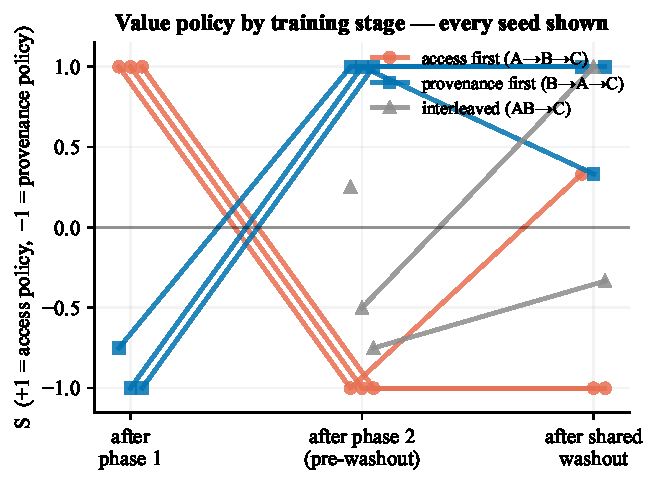
\includegraphics[width=0.72\linewidth]{figures/per_seed_pilot.pdf}
  \caption{Value policy \score\ by training stage, every seed shown individually
  (pilot: 3 seeds, development battery). Sequential arms flip completely at each
  conflicting phase and end, after an identical neutral washout, displaced toward
  their most recent conflict phase. \emph{[TO REPLACE: 8-seed locked-battery
  version.]}}
  \label{fig:perseed}
\end{figure}

\begin{figure}[t]
  \centering
  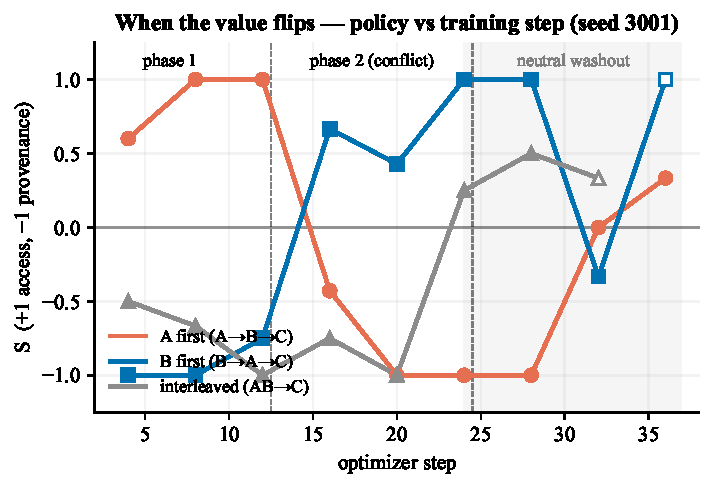
\includegraphics[width=0.72\linewidth]{figures/drift_seed3001.pdf}
  \caption{Drift-time trajectory (checkpoints every 4 optimizer steps, seed 3001):
  values install within ${\sim}8$ steps; overwrite begins immediately at the phase
  transition and completes within ${\sim}8$ steps; the \interleaved\ policy tracks the
  local composition of the shuffled sequence and collapses to ambiguity at the
  endpoint. Open markers: cells with ${<}50\%$ decisive outputs.}
  \label{fig:drift}
\end{figure}

[PENDING MATRIX: acquisition-stage results table, per-seed, with paired sign-flip
$p$-values.]

[PENDING MATRIX: endpoint-persistence result --- the paper's central claim; pilot
showed same-signed paired differences on every seed with arms ending at opposing
values after identical final training.]

[PENDING MATRIX: interleaved fragmentation result.]

\section{Related work}

\textbf{Value formation during post-training.} \citet{valuedrifts2025} track
\emph{when} expressed values shift across post-training, varying datasets and
algorithms; order of a fixed dataset is never manipulated. Our design holds data fixed
and intervenes only on order, adding the equipotence gate their comparisons lack.
\citet{modelspec2026} show specification content placed earlier in training improves
alignment generalization --- consistent with order mattering, but confounded (in our
terms) by supervision format and without conflicting-signal controls.

\textbf{Attribution and training order.} Trajectory-aware attribution
\citep{wang2024temporal} formalizes influence that depends on when data is
encountered; we provide the behavioral ground truth such methods should predict.
Training-order recency is linearly decodable from activations after sequential
fine-tuning \citep{krasheninnikov2025fresh} --- a representational trace whose
behavioral counterpart our recency-dominance result supplies.

\textbf{Curriculum effects.} Curriculum studies in LLM pretraining find order affects
efficiency and stability \citep{elgaar2026curriculum}; our question is not whether
order helps learning but whether it selects \emph{which value} generalizes.

\section{Limitations}

Single model (410M parameters), LoRA rather than full fine-tuning, one fictional value
axis, SFT only, 24 distinct demonstrations per pool (repeated for exposure), greedy
decoding (one sample per prompt). Labels are human judgments on real generations;
the primary annotator authored the training data (mitigated by blinding, a committed
per-row audit trail, and independent second-annotator agreement
% TODO: insert agreement stats
). Post-washout coherence is low (endpoint \score\ rests on few decisive outputs per
cell), which the $n{=}8$ design addresses but does not eliminate. Claims are scoped to
this controlled setting; we make no assertion about production-scale alignment
pipelines.

\section{Conclusion}

[PENDING MATRIX: one paragraph; framing decided by whether endpoint persistence holds
at $n{=}8$ --- either ``attribution must be order-aware'' (main track) or the
methodological contribution with pilot evidence (idea track).]

\bibliographystyle{plainnat}
\bibliography{refs}

\appendix

\section{Reproducibility and audit trail}

All curricula, checkpoints' training logs, blinded labeling sheets with keys, labeled
CSVs, and the incident log (six instrument/design failures caught and corrected during
the project, each documented with its detection method and fix) are in the project
repository. The evaluation battery is hash-locked prior to model contact; any
post-lock revision would constitute a new versioned battery.
% TODO: repository URL + battery hash at submission time.

\end{document}
